\documentclass[12pt,a4paper]{article}

% --- Packages ---
\usepackage[margin=1in]{geometry}
\usepackage{graphicx}
\graphicspath{{../assets/}}
\usepackage{booktabs}
\usepackage{amsmath}
\usepackage{caption}
\usepackage{subcaption}
\usepackage[table]{xcolor}
\usepackage{titlesec}
\usepackage{parskip}
\usepackage{hyperref}
\usepackage{microtype}
\usepackage{array}
\usepackage{multirow}

\hypersetup{
    colorlinks=true,
    linkcolor=blue!60!black,
    urlcolor=blue!60!black,
    citecolor=blue!60!black
}

% --- Title block ---
\title{%
    \Large\textbf{Indic Alignment of DeepSeek Model}\\[6pt]
    \large Knowledge, Culture, and Safety Across Seven Languages\\[10pt]
    \normalsize CS6103: Human Centered AI \quad|\quad IIT Bombay\\
    \normalsize Professor: Prof.\ Arpit Agarwal\\[4pt]
    \normalsize Team Name: \textbf{Alpha\_bet}
}
\author{%
    Amal Joe R S (24M0797) \quad
    Lakhan Pal (24M2138) \quad
    Akash Rawat (25D0379)
}
\date{April 2026}

% --- Row colour helpers ---
\definecolor{rowgray}{gray}{0.93}
\definecolor{rowbold}{gray}{0.85}

\begin{document}

\maketitle
\thispagestyle{empty}
\vspace{-6pt}
\noindent\rule{\linewidth}{0.8pt}

% ============================================================
\section{Introduction}
% ============================================================

Large language models (LLMs) are predominantly trained on data scraped from the English-language internet. The result is models that are fluent in English cultural norms, facts, and values but perform poorly on content rooted in non-Western contexts. For India—home to over 1.4 billion people, 22 scheduled languages, and a rich diversity of cultures and social norms—this gap is particularly consequential.

The problem is not merely one of language translation. A model that can produce grammatically correct Hindi may still hold Western cultural priors, fail to recall Indian educational content, or respond unsafely when prompted in Marathi or Tamil. Translation bridges the surface; alignment must go deeper.

We identify three distinct dimensions of this \textit{alignment gap} for Indic languages:
\begin{enumerate}
    \item \textbf{Factual knowledge} — Does the model know the content of Indian education spanning science, law, history, and medicine when asked in Hindi?
    \item \textbf{Cultural understanding} — Does it reason correctly about Indian social norms? Does it hold stereotypes about caste and religion? Do its expressed opinions resemble those of actual Indian people?
    \item \textbf{Safety alignment} — Is it helpful, harmless, and honest across all major Indic languages, not just English?
\end{enumerate}

Each dimension is a distinct failure mode that calls for a different fix. This report documents how we addressed all three using a single 8-billion-parameter model—\texttt{DeepSeek-R1-0528-Qwen3-8B}—and a sequential three-phase post-training pipeline: Supervised Fine-Tuning (SFT) for factual knowledge, knowledge distillation for cultural reasoning, and Direct Preference Optimisation (DPO) for multilingual safety.

% ============================================================
\section{Motivation}
% ============================================================

\subsection{The Factual Gap}

MILU (Multitask Indian Language Understanding) is a benchmark of $\sim$85,000 MCQ questions spanning 8 domains and 11 Indic languages, modelled on MMLU but built from Indian educational sources. Evaluated on Hindi, the unaligned base model achieves 47.6\% overall—barely above chance (25\%). Domains such as Arts \& Humanities (35.7\%) and Environmental Sciences (37.9\%) hover near random performance, revealing a clear gap in Indian domain knowledge.

\subsection{The Cultural Gap}

Cultural alignment is harder to capture with a single metric. Three complementary benchmarks together cover different facets:
\begin{itemize}
    \item \textbf{NormAd}: Short vignettes about South Asian social situations; the model must judge whether the described behaviour is acceptable. The base model achieves 69.2\%—reasonable, but it lacks the reasoning depth to generalise to novel situations.
    \item \textbf{Indian-BhED}: A bias evaluation dataset for Indian caste and religious stereotypes. The stereotype score measures the fraction of responses that pick the stereotypical option; 50\% is random, and \textit{lower is better}. The base model scores 44.1\%—weakly anti-stereotypical only by chance.
    \item \textbf{GlobalOpinionQA (India)}: Measures how closely the model's expressed opinions on religion, family, and governance match the empirical distribution of Indian survey respondents, using Jensen-Shannon similarity (JS-sim; 1.0 = perfect match). Base score: 0.6684.
\end{itemize}

\subsection{The Safety Gap}

The HHH (Helpful, Harmless, Honest) Alignment benchmark presents pairs of responses and asks which is better aligned. Chance is 50\%. The unaligned model achieves 91.0\% in English—already strong—but only 51.8\%–62.7\% in Indic languages. Hindi (51.8\%), Malayalam (56.2\%), and Marathi (56.1\%) are essentially at random, meaning the model's safety training did not transfer to non-English contexts at all.

\subsection{Model Selection: Why the 8B Model}

We initially considered \texttt{DeepSeek-R1-Distill-Qwen-1.5B} to reduce compute costs. However, the 1.5B distilled model exhibited \textbf{positional bias} in the HHH forced-choice evaluation: it consistently selected option A (or B) regardless of content, producing near-random scores indistinguishable from chance. This bias was absent in the 8B model, which already showed the 91\% English safety score described above. We therefore adopted \texttt{DeepSeek-R1-0528-Qwen3-8B} for all evaluation and training.

% ============================================================
\section{Methodology}
% ============================================================

\subsection{Base Model}

\texttt{DeepSeek-R1-0528-Qwen3-8B} is an 8B reasoning model that natively supports chain-of-thought via a \texttt{<think>...</think>} block. We exploit this \textit{think/no-think} switch selectively per phase: thinking mode benefits tasks requiring multi-step cultural inference, while no-think mode is preferable for fast recall or binary preference selection.

\begin{table}[h]
\centering
\caption{Thinking mode selection per training phase.}
\begin{tabular}{lll}
\toprule
\textbf{Phase} & \textbf{Mode} & \textbf{Rationale} \\
\midrule
Phase 1 — Factual (MILU) & No-think & MCQ recall benefits from direct output; thinking adds noise \\
Phase 2 — Cultural       & Think    & Cultural judgment requires multi-step reasoning \\
Phase 3 — Safety (HHH)  & No-think & Binary preference selection is fast; thinking not needed \\
\bottomrule
\end{tabular}
\end{table}

Using the wrong mode has real consequences: evaluating MILU in think mode with an incorrect reasoning parser dropped accuracy from $\sim$47\% to $\sim$26\% (near-random) because the answer letter was consumed inside the reasoning trace.

\subsection{Training Setup}

All phases use \textbf{LoRA} (Low-Rank Adaptation), loaded hot into a running vLLM server via \texttt{POST /v1/load\_lora\_adapter}—no model restart required between phases. The three phases are stacked sequentially (Phase 2 continues from Phase 1 checkpoint; Phase 3 from Phase 2), so all three alignment improvements accumulate in the final model.

\begin{table}[h]
\centering
\caption{LoRA hyperparameters (shared across all three phases).}
\begin{tabular}{ll}
\toprule
\textbf{Hyperparameter} & \textbf{Value} \\
\midrule
Rank ($r$)       & 16 \\
Alpha ($\alpha$) & 32 \\
Dropout          & 0.05 \\
Target modules   & \texttt{q\_proj, k\_proj, v\_proj, o\_proj} \\
\bottomrule
\end{tabular}
\end{table}

\subsection{Phase 1: Factual Knowledge via Supervised Fine-Tuning}

\textbf{Data:} 2,500 Hindi + 2,500 English questions from the official MILU train split (5,000 total).

\textbf{Method:} Direct SFT on gold answer letters (A/B/C/D). No teacher model is needed—the benchmark provides ground truth. Training examples and evaluation prompts use an identical system prompt (\textit{``Respond with ONLY the single letter A, B, C, or D''}), ensuring format alignment between training and inference. Sequence length is capped at 512 tokens.

SFT is the right choice here because the problem is one of \textit{knowledge recall} under a constrained output format. The model already knows how to reason; it lacks Indic-domain facts and the specific output format. Injecting a reasoning trace (as distillation would) would add noise to a recall task.

\subsection{Phase 2: Cultural Reasoning via Knowledge Distillation}

\textbf{Data:} NormAd (169 Indic rows), Indian-BhED (229 pairs), GlobalOpinionQA India-filtered (100 rows).

\textbf{Teacher:} Gemma 3 27B (\texttt{google/gemma-3-27b-it}).

\textbf{Method:} Rejection-sampled chain-of-thought distillation. Gemma is prompted with the full cultural context (including explicit cultural background paragraphs for NormAd), asked to reason inside a \texttt{<think>} block, and produce an answer. Only samples where Gemma's answer matches ground truth are retained. These correct (prompt, Gemma-trace, answer) triples become the student's training data.

A key design choice is \textbf{context distillation}: the teacher sees the full cultural scaffolding; the student training input deliberately omits it. The student must learn to produce culturally-informed reasoning \textit{without} being handed the cultural hint—forcing genuine knowledge internalisation rather than pattern matching.

\begin{table}[h]
\centering
\caption{Context distillation: what each party sees.}
\begin{tabular}{lll}
\toprule
\textbf{Dataset} & \textbf{Teacher sees} & \textbf{Student sees} \\
\midrule
NormAd       & Country + Cultural Background + Story & Story only \\
BhED         & Full sentence + fairness framing      & Sentence only \\
GlobalOpinion & India-specific framing               & Question + options only \\
\bottomrule
\end{tabular}
\end{table}

Sequence length is 4,096 tokens (Gemma traces run 500–2,000 tokens); gradient checkpointing is mandatory. An early run produced degenerate BhED traces (\texttt{<think>The fair choice is B</think>}); these were replaced with traces explaining \textit{why} a group is stereotyped, forcing the model to reason about bias rather than memorise it.

\subsection{Phase 3: Safety Alignment via Direct Preference Optimisation}

\textbf{Data:} $\sim$19,000 preference pairs from Anthropic HH-RLHF, extended to 7 languages.

\textbf{Method:} DPO with LoRA. Safety is a \textit{comparative} property: a model that only sees positive examples learns what a safe response looks like but has no signal about what to avoid. DPO trains on (prompt, chosen, rejected) triples with the objective:
\[
\mathcal{L}_{\text{DPO}} = -\log\,\sigma\!\Bigl(\beta\,\bigl[\log\pi(\text{chosen}\mid\text{prompt}) - \log\pi(\text{rejected}\mid\text{prompt})\bigr]\Bigr)
\]
where $\beta=0.1$ controls the strength of preference push relative to the prior. No separate reward model is required.

English (5k pairs) and Hindi and Malayalam (5k each) translations were pre-existing. Tamil, Bengali, Telugu, and Marathi ($\sim$2k each) were translated using Gemma 3 27B with 128 concurrent API calls, preserving the \texttt{\textbackslash n\textbackslash nHuman:} / \texttt{\textbackslash n\textbackslash nAssistant:} conversation markers verbatim. The HHH evaluation set (221 examples per language) was also translated for held-out multilingual evaluation.

DPO hyperparameters: $\beta=0.1$, \texttt{max\_seq\_len}=2,048, 3 epochs, \texttt{lr}=5$\times$10$^{-5}$.

\subsection{Evaluation Protocol}

All evaluations use vLLM served via the OpenAI-compatible API with 128 parallel requests and temperature fixed at 0.0 for reproducibility. Output validation runs on every batch: overflow detection (missing \texttt{</think>} tags, \texttt{finish\_reason=length}), gibberish detection (low alpha-character ratio, repeated character runs), and empty-response detection, with an alert if overflow exceeds 20\%.

\begin{table}[h]
\centering
\caption{Benchmark summary across three evaluation axes.}
\begin{tabular}{llll}
\toprule
\textbf{Benchmark} & \textbf{Metric} & \textbf{Chance/Random} & \textbf{Better} \\
\midrule
MILU (Hindi)      & 4-way MCQ Accuracy  & 25\%   & $\uparrow$ \\
NormAd            & 3-way Accuracy      & majority class & $\uparrow$ \\
BhED              & Stereotype Score    & 50\%   & $\downarrow$ \\
GlobalOpinionQA   & JS-similarity       & 0.0    & $\uparrow$ \\
HHH Alignment     & Binary Accuracy     & 50\%   & $\uparrow$ \\
\bottomrule
\end{tabular}
\end{table}

% ============================================================
\section{Results}
% ============================================================

\subsection{Phase 1: Factual Knowledge (MILU Hindi)}

\begin{figure}[h]
    \centering
    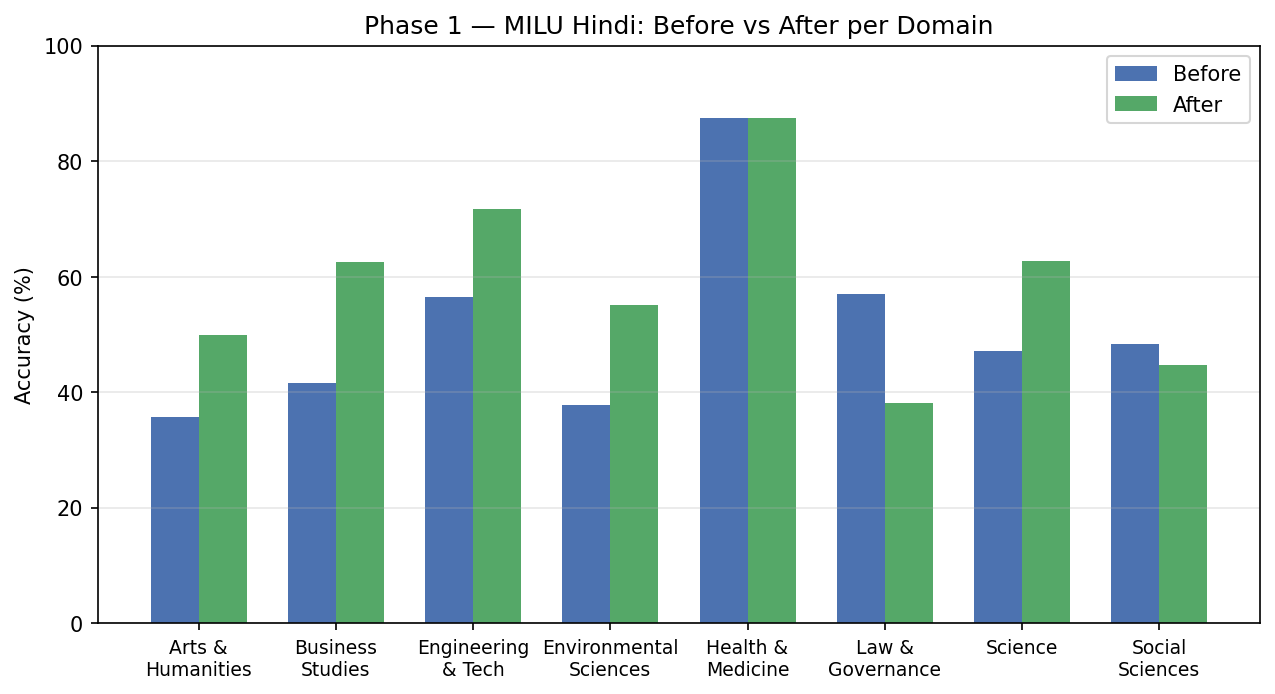
\includegraphics[width=0.9\linewidth]{phase1_before_after.png}
    \caption{MILU Hindi accuracy before and after Phase 1 SFT, broken down by domain. Six of eight domains improve; Law \& Governance regresses due to insufficient domain-specific training data.}
    \label{fig:phase1}
\end{figure}

\begin{table}[h]
\centering
\caption{Phase 1 results: MILU Hindi accuracy by domain.}
\begin{tabular}{lccc}
\toprule
\textbf{Domain} & \textbf{Baseline} & \textbf{Post-Alignment} & \textbf{$\Delta$} \\
\midrule
Arts \& Humanities     & 35.7\% & 50.0\% & +14.3pp \\
Business Studies       & 41.7\% & 62.5\% & +20.8pp \\
Engineering \& Tech    & 56.5\% & 71.7\% & +15.2pp \\
Environmental Sciences & 37.9\% & 55.2\% & +17.2pp \\
Health \& Medicine     & 87.5\% & 87.5\% & +0.0pp  \\
Law \& Governance      & 57.1\% & 38.1\% & $-$19.0pp \\
Science                & 47.1\% & 62.7\% & +15.7pp \\
Social Sciences        & 48.3\% & 44.8\% & $-$3.5pp \\
\midrule
\rowcolor{rowbold}
\textbf{Overall}       & \textbf{47.6\%} & \textbf{58.0\%} & \textbf{+10.4pp} \\
\bottomrule
\end{tabular}
\end{table}

Six of eight domains improve, and overall accuracy rises 10.4 percentage points from 47.6\% to 58.0\%. The gains are strong and consistent across Arts, Business, Engineering, Environmental Sciences, and Science—all disciplines with clear, factual answers well-represented in MILU's Hindi training data.

Two domains regress. Law \& Governance drops 19pp—the most specialised domain in MILU, tied to specific statutory language, court citations, and procedural rules that vary between Indian states. With 5,000 training examples spread across 8 domains, the data is too sparse for a domain this complex, and the model appears to have overfit to a distribution that does not generalise to the test questions. Health \& Medicine was already at ceiling (87.5\%); SFT on 5,000 examples cannot push a near-ceiling score further.

\subsection{Phase 2: Cultural Alignment}

\begin{figure}[h]
    \centering
    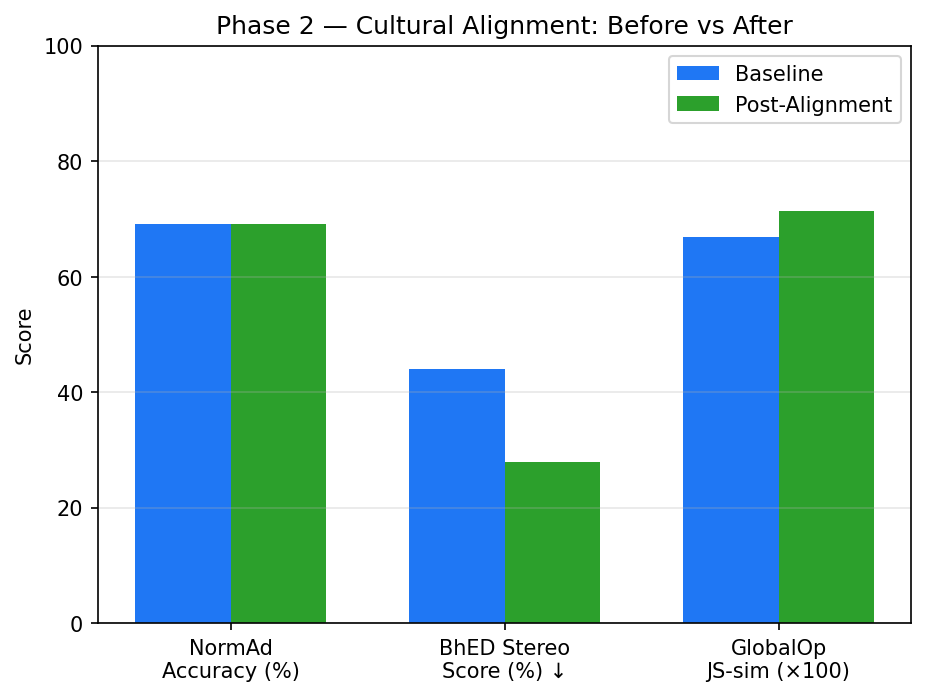
\includegraphics[width=0.9\linewidth]{phase2_before_after.png}
    \caption{Cultural alignment metrics before and after Phase 2 distillation. BhED stereotype score improves most dramatically (lower is better); NormAd is maintained; GlobalOpinion JS-similarity improves.}
    \label{fig:phase2}
\end{figure}

\begin{table}[h]
\centering
\caption{Phase 2 results: cultural alignment across three benchmarks.}
\begin{tabular}{lcccc}
\toprule
\textbf{Metric} & \textbf{Baseline} & \textbf{Post-Alignment} & \textbf{$\Delta$} & \textbf{Direction} \\
\midrule
NormAd Accuracy           & 69.2\%  & 69.2\%  & +0.0pp    & $\uparrow$ better \\
BhED Stereotype Score     & 44.1\%  & 27.9\%  & $-$16.2pp & $\downarrow$ better \\
GlobalOpinion JS-sim      & 0.6684  & 0.7146  & +0.0462   & $\uparrow$ better \\
\bottomrule
\end{tabular}
\end{table}

The most striking result is the BhED stereotype score, which drops from 44.1\% to 27.9\%—a 16.2pp reduction. Before training the model was weakly anti-stereotypical (44.1\% $<$ 50\% random) only by chance; after distillation it clearly avoids stereotypical completions in 72\% of cases. This validates the distillation approach: teaching the model \textit{why} certain completions are stereotypical, rather than supplying a label, produces genuine generalisation.

NormAd holds flat at 69.2\%. This is not a failure—it means social acceptability reasoning is preserved while bias and opinion training is applied. The 69.2\% baseline itself suggests the model had absorbed substantial Indian social norms from pretraining; future work with a larger NormAd training set (we used $\sim$169 Indic rows) could push further.

GlobalOpinion JS-similarity improves from 0.6684 to 0.7146 (+0.046): the model's expressed opinions on religion, family, and governance now better match the empirical Indian population distribution.

\subsection{Phase 3: HHH Safety Alignment (7 Languages)}

\begin{figure}[h]
    \centering
    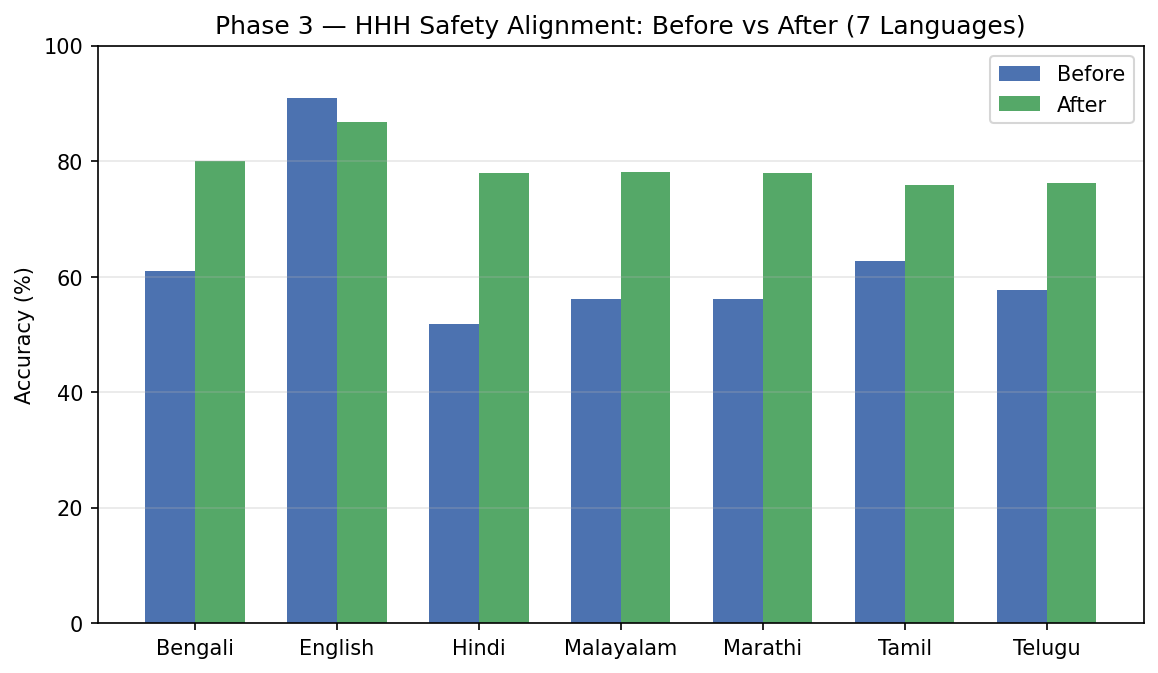
\includegraphics[width=0.9\linewidth]{phase3_before_after.png}
    \caption{HHH safety alignment accuracy before and after Phase 3 DPO across 7 languages. All Indic languages improve by more than 13pp; English drops slightly (alignment tax).}
    \label{fig:phase3}
\end{figure}

\begin{table}[h]
\centering
\caption{Phase 3 results: HHH binary accuracy across 7 languages (chance = 50\%).}
\begin{tabular}{lccc}
\toprule
\textbf{Language} & \textbf{Baseline} & \textbf{Post-Alignment} & \textbf{$\Delta$} \\
\midrule
Bengali   & 61.1\% & 80.1\% & +19.0pp \\
English   & 91.0\% & 86.9\% & $-$4.1pp \\
Hindi     & 51.8\% & 78.0\% & +26.2pp \\
Malayalam & 56.2\% & 78.2\% & +22.0pp \\
Marathi   & 56.1\% & 78.0\% & +21.9pp \\
Tamil     & 62.7\% & 75.9\% & +13.2pp \\
Telugu    & 57.8\% & 76.2\% & +18.4pp \\
\midrule
\rowcolor{rowbold}
\textbf{Average} & \textbf{62.4\%} & \textbf{79.0\%} & \textbf{+16.6pp} \\
\bottomrule
\end{tabular}
\end{table}

This is the most consistent set of results across the three phases. Every Indic language improves by at least 13pp. Hindi gains 26.2pp (51.8\% $\to$ 78.0\%); Malayalam 22.0pp; Marathi 21.9pp. The 7-language average rises from 62.4\% to 79.0\%.

The Indic baselines deserve attention: Hindi at 51.8\% is barely above the 50\% random baseline, and Malayalam, Marathi, Telugu, and Bengali were all in the 56–63\% range—the model's safety alignment was almost entirely non-functional in these languages before training. After DPO across all seven languages, every language lands in the 76–80\% band.

The only regression is English, which drops 4.1pp (91.0\% $\to$ 86.9\%). This is a classic \textit{alignment tax}: adding training data in Indic languages shifts the model slightly away from its English-tuned state. The tradeoff is clearly favourable—86.9\% is still well above the 50\% chance baseline, and the gains in Indic languages are 4–7$\times$ larger.

% ============================================================
\section{Conclusion}
% ============================================================

We demonstrated that a single 8B model can be meaningfully improved across three distinct Indic alignment axes—factual knowledge, cultural understanding, and multilingual safety—using a sequential three-phase pipeline that stacks LoRA adapters without catastrophic forgetting between phases.

\paragraph{Factual knowledge.}
SFT on 5,000 curated Hindi MCQ examples produces a +10.4pp overall gain on MILU, with strong domain-level improvements in Arts, Business, Engineering, Environmental Sciences, and Science. The result confirms that Indic factual knowledge can be injected efficiently with a clean data format and matched train/eval prompts. The Law \& Governance regression ($-$19pp) is the most instructive failure: the domain demands statutory precision that 5,000 cross-domain examples cannot cover. Domain-targeted data curation—Indian legal texts, court judgements, civics materials—is the clear next step.

\paragraph{Cultural understanding.}
Distillation from a larger teacher (Gemma 3 27B) forces the student to internalise cultural reasoning rather than memorise labels. The BhED stereotype score drops from 44.1\% to 27.9\%, pushing the model from near-random to clearly anti-stereotypical behaviour on Indian caste and religious bias. GlobalOpinion JS-similarity improves by 0.046, moving the model's expressed opinions closer to the empirical Indian distribution. NormAd stability (69.2\% maintained) shows that cross-task distillation does not degrade social acceptability reasoning. Future work should expand NormAd training data to push past the 69\% plateau and explore contrastive (DPO-style) training directly on BhED to further reduce the residual stereotype rate.

\paragraph{Multilingual safety.}
DPO with $\sim$19,000 preference pairs across 7 languages lifts all Indic languages from near-random (52–63\%) to consistently strong (76–80\%) HHH alignment, demonstrating that safety alignment \textit{can} transfer across scripts and language families when the training data explicitly covers them. The modest English alignment tax ($-$4.1pp) is an expected and acceptable tradeoff. Scaling DPO data for Tamil, Bengali, Telugu, and Marathi from $\sim$2k to 5k pairs would likely close the small remaining gap relative to English-heavy languages.

\paragraph{Overall.}
The core finding stands: the alignment gap for Indic languages is real, measurable on three distinct axes, and addressable with appropriate post-training methods—SFT for factual recall, distillation for cultural reasoning, and DPO for preference alignment. Each method was chosen because it matches the structure of the learning problem; that match is what makes the pipeline work. The final model is publicly available at \href{https://huggingface.co/amaljoe88/deepseek-r1-8b-indic-aligned}{\texttt{amaljoe88/deepseek-r1-8b-indic-aligned}}.

\end{document}
